\label{cap_trabajos_relacionados}
\chapter{Trabajos Relacionados}
En este capítulo se describen brevemente aquellos algoritmos y herramientas propuestas existentes que fueron investigadas durante el transcurso de este trabajo. Algunas de ellas son herramientas que incluyen algoritmos de layout incorporados, otras brindan interfaces de prueba que nos permiten ver el funcionamiento de los algoritmos teorizados, y por otro lado algunos simplemente diseñan los algoritmos o metodologías pero no presentan una implementación.

Las implementaciones consideradas son las siguientes: 

% En este capítulo se describen brevemente aquellas herramientas y propuestas existentes que
% fueron investigadas durante el transcurso de este trabajo. Algunas de ellas permiten la creación y
% edición de modelos de variabilidad y su posterior análisis automático con el objeto de validarlos.
% Mientras que otras solo proponen nuevos métodos de formalización de dichos modelos. Este
% análisis ha sido realizado teniendo en cuenta los siguientes aspectos: soporte gráfico para el
% modelado, lenguaje de modelado de variabilidad, los métodos de formalización de los diagramas,
% el uso de razonamiento para validar modelos y, en caso que sea posible, cuán integrados trabajan
% el soporte gráfico y el razonamiento automático.
% Las implementaciones consideradas son las siguientes: FaMa-OVM [13], S.P.L.O.T [41], VariaMos
% [19]. Otras propuestas en consideración que no presentan implementación son: [5, 42].

\section{Algoritmo de Fuerzas de Tunkelang}
Uno de los algoritmos mas conocidos para layout de grafos genéricos es el Algoritmo Dirigido por Fuerzas de Tunkelang \cite{tunkelang1998jiggle}. Este algoritmo  propone un modelo físico donde los nodos y arcos realizan fuerzas de repulsión entre ellos para evitar cruzamientos. Esta simulación se realiza por un tiempo dado hasta obtener el resultado deseado. En este la eficacia del resultado está ligada a las posiciones iniciales del grafo de entrada y, en este sentido, a la densidad o separación de sus nodos y arcos.

Este algoritmo no presenta una visualización simétrica de los nodos y es mas efectivo para grafos dispersos. Se han hecho pruebas satisfactorios con grafos de hasta unos 60 nodos \cite{gibson2013survey}.

\begin{figure*}[h]
	\centering
	\subfigure[Grafo original generado aleatoriamente.]{
		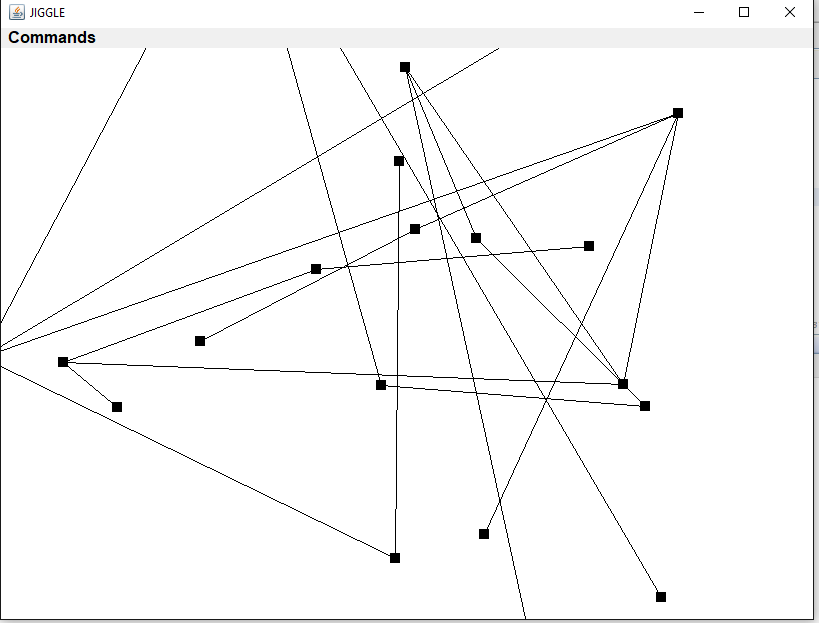
\includegraphics[width=7cm]{imagenes/jiggle_1.png}
		\label{subfig:jiggle_1}
	}
	\subfigure[Grafo luego de utilizar el algoritmo dirigido por fuerzas.]{
		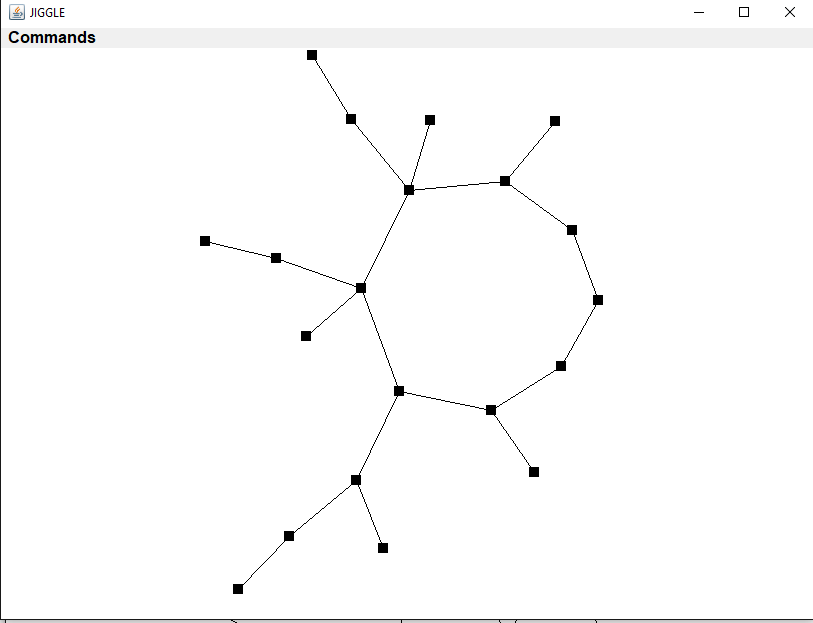
\includegraphics[width=7cm]{imagenes/jiggle_2.png}
		\label{subfig:jiggle_2}
	}
	\caption{Ejemplo de layout de grafo utilizando la herramienta Jiggle que provee Tunkelang para probar sus algoritmos.}
	\label{fig:jiggle}
\end{figure*}

% En el survey de Helen Gibson et al. \cite{gibson2013survey} se han recopilado gran variedad de algoritmos de layout, de los cuáles el más adecuado, con respecto a precisión y velocidad, para layout en modelado conceptual, es el algoritmo Dirigido por Fuerzas de Tunkelang \cite{tunkelang1998jiggle}. Este algoritmo  propone un modelo físico donde los nodos y arcos realizan fuerzas de repulsión entre ellos para evitar cruzamientos. Esta simulación se realiza por un tiempo dado hasta obtener el resultado deseado. En este la eficacia del resultado está ligada a las posiciones iniciales del grafo de entrada.

\section{Algoritmos Genéticos de Layout: TimGA y Hongmei He}
Los algoritmos de TimGA \cite{eloranta2001timga} utilizan grafos genéricos, es decir sin ninguna disposición particular de los nodos y arcos, para representar los individuos de sus algoritmos genéticos, como se muestra en la figura \ref{fig:timga_representacion}. En general este esquema de representación de individuos produce que las operación de variación que se tengan que definir sean mas complejas que con otras representaciones mas simples, y por lo tanto la computación del algoritmo se ve demorada.

Las pruebas realizadas sobre estos algoritmos han dado tiempos considerables para alcanzar un máximo local o global, debido a la gran variabilidad que existe entre grafos sin ningún estilo de dibujado particular \cite{gibson2013survey} (ver sección \ref{sec:estilos_de_dibujado}).

\begin{figure}[H]
	\centering
	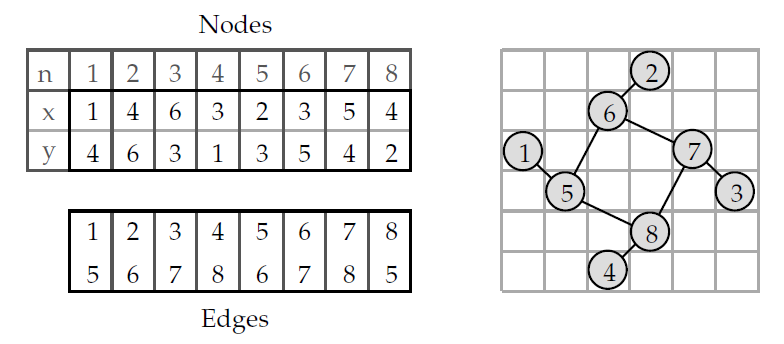
\includegraphics[width=13cm]{imagenes/timga_representacion.png}
	\caption{Representación de individuos en TimGA \cite{eloranta2001timga}.}
	\label{fig:timga_representacion}
\end{figure}

Por otro lado Hongmei He \cite{he2007parallelisation} utiliza para representar a sus individuos un estilo de dibujado de diagrama de arcos (ver sección \ref{sec:dibujado_diagrama_de_arcos}) y busca que la implementación del algoritmo permita utilizar paralelismo para agilizar su computación. A pesar de esto, los resultados que obtiene manejan tiempos considerables para la práctica debido en gran medida a que el grafo inicial del que parten para la generación de la población inicial es aleatorio y en ciertos casos puede llevar mucho tiempo alcanzar un máximo local \cite{gibson2013survey}.

Ambos algoritmos consideran como parámetro principal para evaluar el fitness de sus individuos el crossing number de estos (ver sección \ref{sec:crossing_number}).

% Por otro lado, otros algoritmos desarrollados para diagramas  genéricos que  utilizan métodos adaptativos, como por ejemplo algoritmos genéticos  \cite{eloranta2001timga, he2007parallelisation},  tienen problemas por la  considerable cantidad de generaciones que deben analizar, lo que conlleva a que  se consuma un tiempo elevado en alcanzar un máximo local o global. 
	
\section{Plugins de Layout para Protégé: OntoGraph, OWLViz y SOVA}
Protégé \cite{knublauch2004protege} incluye entre sus plugins pre-instalados, utilidades de visualización de ontologías como son OntoGraph \cite{falconer2010ontograf}[Fig. \ref{fig:ontograph}] y OWLViz \cite{horridge2010owlviz} [Fig. \ref{fig:owlviz}]. Estos brindan la capacidad a Protégé de visualizar una ontología en lenguaje OWL como un árbol, con conectores que simbolizan las relaciones de subsunción y las equivalencias entre las clases.

\begin{figure}[h]
	\centering
	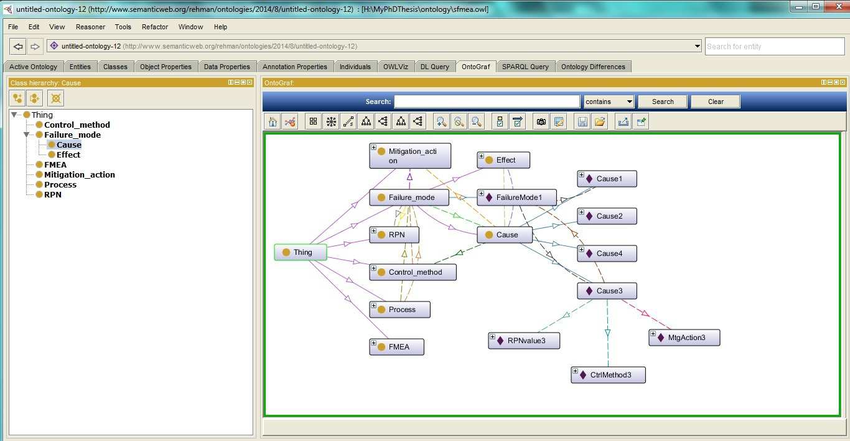
\includegraphics[width=13cm]{imagenes/ontograph.png}
	\caption{Herramienta Protégé utilizando el plugin OntoGraph sobre una ontología en OWL.}
	\label{fig:ontograph}
\end{figure}

Los algoritmos de layout que disponen incluyen una distribución en forma de árbol descendiente o lateral. En el caso de OntoGraph también incluye un algoritmo de layout basado en un sistema de resortes (Spring Systems) \cite{kobourov2012spring}[Fig. \ref{fig:spring_systems}]. Este algoritmo funciona de manera similar al de dirigido por fuerzas de Tunkelang \cite{tunkelang1998jiggle}, computando fuerzas de atracción entre los nodos adyacentes y fuerzas de repulsión entre todos los pares de nodos.

\begin{figure}[H]
	\centering
	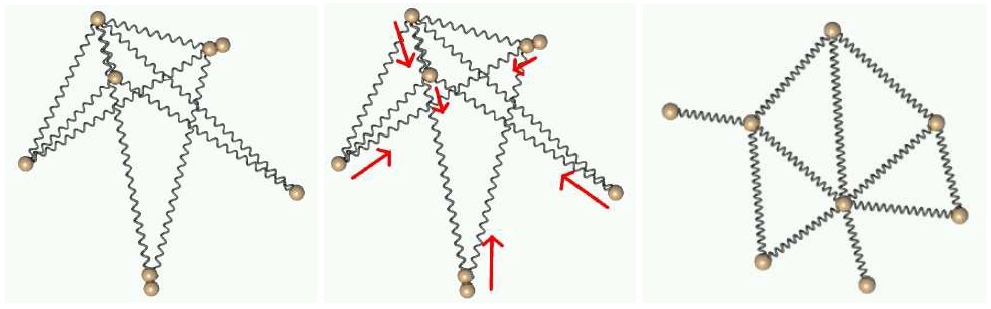
\includegraphics[width=13cm]{imagenes/spring_systems.png}
	\caption{Ilustración de un sistema de resortes genérico: empenzando desde posiciones aleatorias, trata al grafo como un sistema de resortes y busca encontrar una configuración estable \cite{gajer2002grip}.}
	\label{fig:spring_systems}
\end{figure}

\begin{figure}[h]
	\centering
	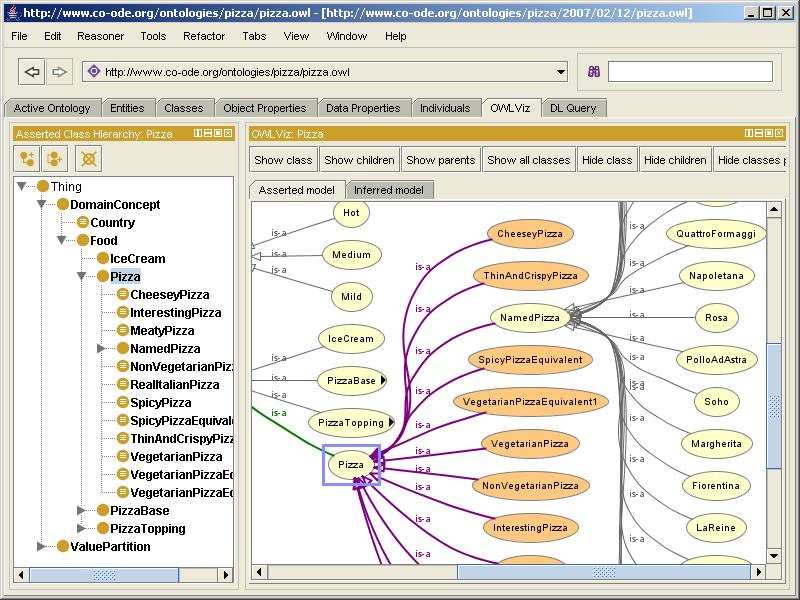
\includegraphics[width=10cm]{imagenes/owlviz.jpg}
	\caption{Herramienta Protégé utilizando el plugin OWLViz sobre una ontología en OWL.}
	\label{fig:owlviz}
\end{figure}

% Illustration of a generic spring embedder: starting from random positions, treat the graph as spring
% system and look for a stable configuration [32].

% This algorithm is similar to that of Eades in that both algorithms compute attractive forces
% between adjacent vertices and repulsive forces between all pairs of vertices

\section{OWLGrEd}
OWLGrEd \cite{liepinvs2014owlgred} es una herramienta de visualización de ontologías OWL, la cuál al momento de renderizar el diagrama utiliza algoritmos de layout. Los diagramas en OWLGrEd utilizan un layout Ortogonal \cite{bekos2012smooth}[Fig. \ref{fig:ortogonal}] sobre las relaciones, a excepción de las relaciones de herencia, las cuales las muestra con un layout jerárquico. Las relaciones de herencia fluyen desde un lado del diagrama hacia el lado opuesto, y las demás relaciones fluyen perpendicularmente a estas, como puede verse en la figura \ref{fig:owlgred}. Esto es debido a que las relaciones de herencia típicas de un diagrama OWL tienden a leerse mas fácilmente de izquierda a derecha y guían a un diagrama mas compacto.

\begin{figure}[h]
	\centering
	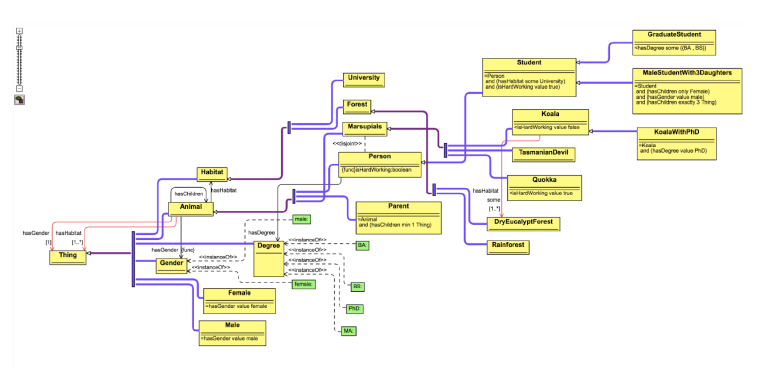
\includegraphics[width=13cm]{imagenes/owlgred.png}
	\caption{Visualización una ontología OWL en OWLGrEd \cite{liepinvs2014owlgred}.}
	\label{fig:owlgred}
\end{figure}

\begin{figure*}[h]
	\centering
	\subfigure[]{
		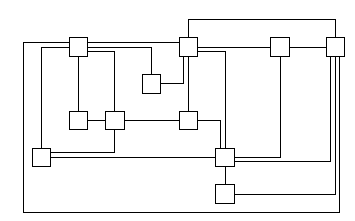
\includegraphics[width=5cm]{imagenes/ortogonal_1.png}
		\label{subfig:ortogonal_1}
	}
	\subfigure[]{
		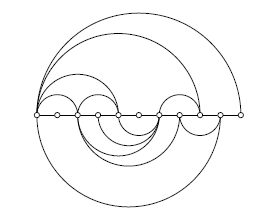
\includegraphics[width=5cm]{imagenes/ortogonal_2.png}
		\label{subfig:ortogonal_2}
	}
	\caption{Ejemplo de un grafo visualizado con un layout ortogonal y con un estilo de diagrama de arcos \cite{bekos2012smooth}.}
	\label{fig:ortogonal}
\end{figure*}

% OWLGrEd diagrams use the orthogonal layout where the inheritance-defining
% relations (i.e. subclass-of relations between classes and instance-of relations
% between classes and instances) are presented in a hierarchical layout (i.e. they
% “flow” from one side of the diagram to the opposite side) and all other relations
% “flow” in the direction perpendicular to it. We have observed that for a typical
% OWL diagram the horizontal direction (left-to-right) seems to be the more
% readable and the one which leads to more compact diagrams.

\section{VOWL}
Los grafos son visualizados en VOWL \cite{lohmann2016visualizing}[Fig. \ref{fig:vowl}] utilizando el algoritmo de layout dirigido por fuerzas. Este layout tiene a ordenar los nodos de tal manera que las clases con mas conexiones este ubicadas mas próximas al centro de la visualización, y viceversa las que tienen menos conexiones mas próximas a la periferia. En este sentido, el layout dirigido por fuerzas ayuda a reflejar la importancia relativa de las clases en el grafo que está siendo visualizado, ya que el número de conexiones de una clase es usualmente un indicador de la importancia que esta tiene en la ontología \cite{peroni2008identifying}.

En VOWL algunos conceptos pueden aparecer multiplicados varias veces como nodos en la visualización del grafo. Esto ayuda a que el layout dirigido por fuerzas no tenga que ser forzado a resolver cruces de arcos complejos, por lo que relaja la visualización y facilita la navegabilidad. Para realizar tal multiplicación, VOWL sigue un conjunto de reglas que determinan que elementos pueden multiplicarse ya sea, para una clase en particular o para el grafo completo.

\begin{figure}[H]
	\centering
	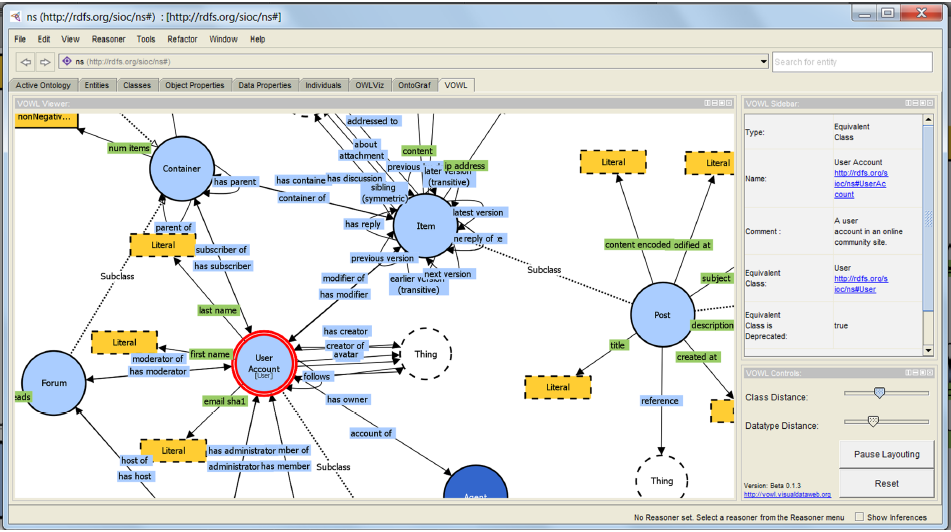
\includegraphics[width=13cm]{imagenes/vowl.png}
	\caption{Interfaz de VOWL que permite visualizar una ontología y posee una barra de herramientas para configurar algunas preferencias. \cite{lohmann2016visualizing}.}
	\label{fig:vowl}
\end{figure}


% By default, VOWL graphs are visualized in
% a force-directed layout. Such a layout tends to arrange
% the nodes in a way that highly connected classes are
% placed more to the center of the visualization, whereas
% less connected ones are placed rather in the periphery.
% Thus, the force-directed layout helps to reflect the relative importance of the classes in the resulting graph
% visualization, as the number of connections of a class
% is often an indication of its importance in the ontology [84]. Moreover, graph layouts created with forcedirected algorithms are perceived to be aesthetically
% pleasant, since all edges have roughly the same length
% and since they tend to avoid edge crossings, which increases the readability of the visualization [5].
% In the same spirit as some elements are merged in
% VOWL, others are multiplied so that they may appear
% more than once in the graph. This helps to relax the
% energy of the force-directed layout and reduces the visual prominence of generic ontology concepts. Multiplication is based on the aforementioned splitting rules
% that determine whether there is no multiplication for
% elements, multiplication for each connected class, or
% multiplication across the entire graph. For instance,
% the generic class owl:Thing is multiplied in a way
% that it is added once for every class it is connected to,
% whereas datatype nodes appear once for every datatype
% property (cf. Figure 1).

% Algunas  herramientas para modelado ontológico tales como OWLViz \cite{horridge2010owlviz}, OntoGraph \cite{falconer2010OntoGraph}, SOVA \cite{kunowski2012sova}, OWLGrEd \cite{cerans2012advanced}, VOWL \cite{lohmann2014protegevowl} e ICOM \cite{fillottrani2012icom}, poseen algoritmos de layout automático, pero con ciertas limitaciones.  En primer lugar, OWLViz, OntoGraph y SOVA son plug-ins de Protégé \cite{knublauch2004protege} que utilizan grafos como lenguaje gráfico para ontologías. Por lo tanto, si bien ofrecen algoritmos visuales, están limitados en cuanto a la expresividad gráfica subyacente. ICOM y OWLGrEd están basados en los lenguajes de modelado conceptual EER y UML, respectivamente. Ambos permiten representar ontologías OWL \cite{hitzler2009owl} y poseen capacidades de layout automático. Sin embargo, solo proveen un conjunto de alineamientos fijos y estáticos. Además, el soporte gráfico de ICOM está actualmente descontinuado. Por último, VOWL también implementa una visualización dinámica pero, al igual que los plug-ins previos, usa grafos como modelos para OWL y no lenguajes de modelado conceptual.

\section{Análisis y Comparación}
El tipo de algoritmos de layout que utilizan OntoGraph, OWLViz, SOVA y OWLGrEd son útiles para grafos planares o de tipo árbol, por lo general para representaciones de ontologías OWL que presentan una jerarquía muy estricta entre sus elementos. Debido a esto, no consideran propiedades de dibujado como el crossing number u optimización de área, si no que se realizan teniendo en cuenta un criterio fijo y estático de organización, debido a que la forma de los grafos siempre será análoga.

En el caso particular de VOWL, este utiliza el algoritmo dirigido por fuerzas, pero nuevamente aprovecha el lenguaje de la representación a su favor, ya que para evitar problemas de cruzamientos multiplica los nodos que generan arcos que rompen la estructura de árbol jerárquica y los coloca en cada nodo como un hijo.

Estos algoritmos cuando queremos aplicarlos sobre modelos conceptuales comienzan a tener complicaciones, debido a la gran variedad de formas que puede tener un grafo para visualizar un diagrama en algún lenguaje de modelado conceptual. En este sentido, se buscaron otro tipo de técnicas mas generales para trabajar sobre layout de grafos, como son las de TimGA y Hongmei He, las cuales atacan el objetivo desde el problema de crossing number, pero sus resultados en la practica tienen complicaciones de eficiencia.

En conclusión, un punto medio entre estas técnicas es lo que se intenta resolver para alcanzar un algoritmo de layout mas óptimo para utilizar sobre diagramas de modelado conceptual.